\documentclass[../../master_thesis_np.tex]{subfiles}
\graphicspath{{./imgs/}}

\begin{document}
\chapter{Discovering Interaction Laws using Machine Learning}
%\todo{machine learning analysis è molto generico... cerca un altro titolo}    
Our goal is to infer the one-body (self-propulsion) and the two-body forces (interactions) that take place in ensembles of active particles using a machine learning tool.
Such systems present a high degree of complexity and a full understanding of the actual interactions has yet to be reached; in this situation, machine learning could be the way of inferring systems' dynamic laws from the observation of simulated and experimental behaviors, with nothing more than some simple assumptions as an underlying model.

As explained in section \ref{literature}, one could use as input some global attribute of the system, such as the radial distribution function, but, as showed by \citeauthor{bag_interaction_2021}, this approach does not work well in out-of-equilibrium cases where an active velocity is present, since when a self-propulsion is present the structure may reflect an attractive interaction applied to an equilibrium case.

\section{Methods}
The tool we propose is based on a Graph Neural Network (GNN) that takes as input the positions and orientations of a set of active particles and tries to predict the resulting velocities.
Here, we tried to replicate the approach used by \citeauthor{ruiz-garcia_discovering_2024}, where a vector of positions and orientations of a set of active particles is given as input to a Graph Neural Network which tries to predict resulting velocities.
Both in our work and in the reference paper the objective is to train a network on simulated data and then use it to predict interaction potential in experiments.
The main difference in in the experimental setup used: \citeauthor{ruiz-garcia_discovering_2024} used snapshots taken from electro-phoretic Janus particles, where some control is held on the system via an external electric field.
This is not the case in the host lab, where autonomous self-diffusio-phoretic Janus particles are used.
Simulation framework is also different: in the reference work particles are simulated using a modified version of LAAMPS \cite{thompson_lammps_2022} molecular dynamics simulator, while our simulation code is made in-house as explained in \ref{chap:int_impl}.

In principle, one could also use a Dense Neural Network (DNN) to learn a high-dimensional nonlinear function that maps a $3N_p$ vector (in 2D, with $N_p$ number of particles) of all particles' positions and orientations into a $2N_p$ vector of velocities, but a Network like this would struggle to adapt to cases with different $N_p$, especially if the number of particles is changing, as happens in experimental settings. 
%\todo{qual è il vantaggio di usare una GNN? spiega}
%\todo{loro lo hanno usato per fare cosa? dati simulati o sperimentali? quali potenziali? spiega}
%\todo{in cosa il nostro lavoro è simile? in cosa è diverso? spiega}

A GNN is structured as a combination of (at most) three DNNs on a graph structure, to predict respectively node (single particle), edge (two particles interactions) and global features.
This way, one could initialize a graph structure at each time step, with nodes storing positions and orientations of particles and undirected, unweighted edges that represent which pairs of particles are considered as interacting.
In principle, such a structure could be initialized with varying number of nodes (particles), since this number does not affect the GNN compatibility, as each edge and node is itself used as input to the network.

\subsection{The Graph Neural Network}
Our GNN is structured as explained in section \ref{literature}, namely with a node and a message function. 
Both of them have 4 layers, with 300 hidden nodes; each hidden layer has a ReLU (Rectified Linear Unit) activation function, while the output layer of each Network is a simple linear layer without any activation.
As for Figure \ref{fig:ruiz1}, the input layer of the message function is $2n_f$ dimensional, where $n_f$ is the number of single particle features, namely $x$, $y$, and $\theta$, to have information about positions and orientations of each pair of interacting agents.
Messages are aggregated using sum as an aggregation function (\verb|'add'| in PyG jargon) to respect the physics of the problem.
The node function's input dimension is $n_f + n_m$ where $n_m$ is the output dimension of the message function; this is done because the node function has the purpose of taking the aggregated message from all the senders (particle inside a threshold distance $\Gamma$) along with the single features of the receiver and trying to predict the receiver's velocity.
In Newtonian dynamics, an acceleration is the result of a force, while in low-Reynolds number regime there is a linear relation between force and velocity.
In this regime, it is convenient to use velocity as a target function to infer force's characteristics.
Overdamped regime is one of the basic assumptions made to build this tool, together with the fact that we neglect many-body interactions, focusing only on one- and two-body forces.
%\todo{ma uno schemino? due equazioni? spiega meglio}
%\todo{approfondisci questo discorso velocità/accelerazione...}

If $\xi$ is the edge function and $\phi$ is the node function (see Figure \ref{fig:ruiz1} as a reference), we have that the predicted velocity $\vec{v}_i^p$ takes the form
\begin{equation}
	\vec{v}_i^p \equiv \tilde{\psi} \left( \vec{c}_i, \sum_{d_{ij} < \Gamma} \vec{\xi} (\vec{c}_i, \vec{c}_j) \right),
\end{equation}
being $\vec{c}_k$ the vector containing positions and orientation of $k$-th particle.
The aim of our network is to minimize the absolute difference between predicted and ground-truth instantaneous velocity, which is our loss function
\begin{equation}
	\mathcal{L} = \sum_{i} \left| \vec{v}_i - \vec{v}_i^p \right|.
\end{equation}

Here it is important to note that the history is not relevant: the network just takes one instant at a time and predicts instantaneous velocities starting from positions and orientations, without knowing what happens before or after.
Ground-truth instantaneous velocities are computed dividing the difference of consecutive positions by the integration time interval, $\frac{\vec{x}(t + \Delta t) - \vec{x}(t)}{\Delta t}$, that is the "right" instantaneous velocity that brings the particle from position $\vec{x}(t)$ at time $t$ to $\vec{x}(t + \Delta t)$.
Since our simulations are performed in periodic boundary conditions, from one frame to the other it can happen that a particle jumps by more than $L$ (side of simulation box), leading to non realistic instantaneous velocities.
After the computation, all velocities get checked and $L/\Delta t$ is subtracted to the ones corresponding to periodic jumps, in order to have physical velocities as ground truth.
%\todo{questo non è chiaro... spiega meglio; mi ricordo che abbiamo ragionato su come calcolare la velocità: spiega il ragionamento e perché è importante, aggiungi equazioni se necessario}

The problem of message dimension $n_m$ is tackled in section \ref{literature}. 
Here, we chose a message dimension $n_m = 2$, as reported in the reference paper \cite{ruiz-garcia_discovering_2024}.
Some trials with $n_m = 100$ and L1 regularization were made, in the spirit of \cite{cranmer_discovering_2020}, but in the message extraction it was not possible to limit the maximum standard deviation to two message components, as, ordering them by variance, the most important components changed from epoch to epoch, not leading to a stable reduction in message size. 
%\todo{perché 2? spiega; in realtà abbiamo provato anche altro, spiega perché alla fine abbiamo scelto 2}

\subsection{Simulations}
To understand the role of the potential's functional form in prediction results, we trained and tested the network on two different simulations, one done using a spring potential with $k_s = \SI{0.1}{\newton\per\meter}$ and $x_0 = \SI{12}{\um}$ and the other using a LJ potential with $\sigma = \SI{4}{\um}$ and $\epsilon = \SI{0.01}{\pico\joule}$.
\todo{aggiungi grafici dei potenziali/forze calcolati con questi parametri}
These potential have the difference in range: without limiting our interaction threshold radius, elastic force not only has effect at long distance but its absolute value increases, while LJ is a short range potential.
In simulations, interaction range is not limited in order to have the maximum amount of interacting particles as possible.
We expect the network to perform worse on LJ since it has less relevant interactions to learn from.

These two potentials required different integration steps: \SI{e-3}{\second} for LJ and \SI{5e-2}{\second} for spring potential.
Both simulations were ran with a particle velocity of \SI{15}{\um \per \second}, in a \qtyproduct{100 x 100}{\um} box with \num{100} particles of \SI{2}{\um} in radius.

\section{Training and Testing}

We let the two systems evolve for a total simulated time of \SI{1000}{\second}, then instantaneous velocities were computed and finally a sample of \num{1000} equally spaced snapshots was taken from each simulation.
We divided these snapshots in \num{750} for training and \num{250} for testing.
The network was trained and tested on each simulation's data separately to have preliminary results.
We tried the same procedure explained in \cite{ruiz-garcia_discovering_2024}, where two particles are considered as linked in the graph if their distance is less than some threshold, and then increasing the threshold in subsequent training loops.
In our case, after learning with the first threshold distance, loss does not decrease and test results do not improve, so what follows refers to a threshold distance of \SI{20}{\um}.
This threshold was chosen in order to have both repulsion and attraction for the two potentials.
In reference paper, only distances up to three particle diameters are plotted in the learned force plots, since no additional information can be extracted from the fast-decreasing potentials \citeauthor{ruiz-garcia_discovering_2024} used.
Lennard Jones is a fast-decreasing potential so it is possible that after this threshold the interaction force is small enough not to have effect on the learning process.
Although elastic force magnitude gets larger with increasing distance, after some time particles will all be oscillating in the vicinity of the equilibrium position $x_0$, leading to a lack of data for larger distances.

After each epoch, the network is used to predict velocities on the test set, which contain data with the same potential used in training, saving the message function outputs.
Then, a minimization process is used to find the best linear transformation that maps message components into the known forces.
This is done to see how results change with the epochs.

\section{Results} \label{4results}
As showed in Figure \ref{fig:learning_curve}, in both cases loss decreases in the 100 epochs of training, meaning that the network is in fact learning.

\begin{figure}[b]
	\centering
	\subfloat{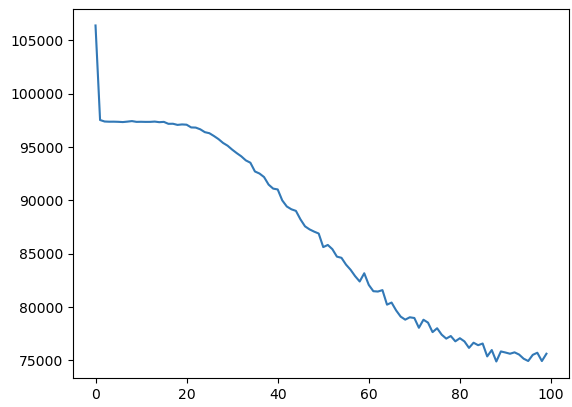
\includegraphics[width=\subfigwidth]{sp_lc.png}}
	\subfloat{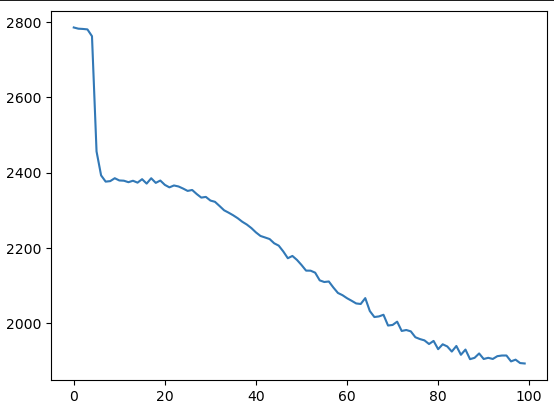
\includegraphics[width=\subfigwidth]{lj_lc.png}}
	\caption{\textbf{NOT DEFINITIVE IMAGES} Learning curve for elastic potential (left) and Lennard Jones (right). Loss is the absolute difference between predicted and ground truth velocities.}
	\label{fig:learning_curve}
\end{figure}

The absolute value of the loss in this case only means that spring potential leads to faster interacting particles and only the decrease is important in our analysis.

Since the output of the message function should represent interaction forces, in order to check the prediction quality we need to compare messages to known forces.
We work in cases where both the distances between particles and the functional form of the force is known, thus we can compute the ground truth.
Here we specify that, since the output of the message function is taken as input by the (linear) node function to predict velocity, it will correspond to the actual force only up to a linear transformation.
A way to compare messages to forces is to compute the ground truth, extract messages from the network and finding the best linear transformation to map one into the other, finding the right parameters that minimize the square difference between the two.
Regarding the message-force plot, a working network with the right linear transformation should show points on the $x = y$ line, being the message components in perfect correspondence with a rotation of the force components as \ref{fig:cranmer1} shows.
In Figure \ref{fig:lincomb} we reported the qualitatively best results, since the loss scoring in this case does not reflect a prediction quality.

\begin{figure}[tp]
	\centering
	\subfloat[][]{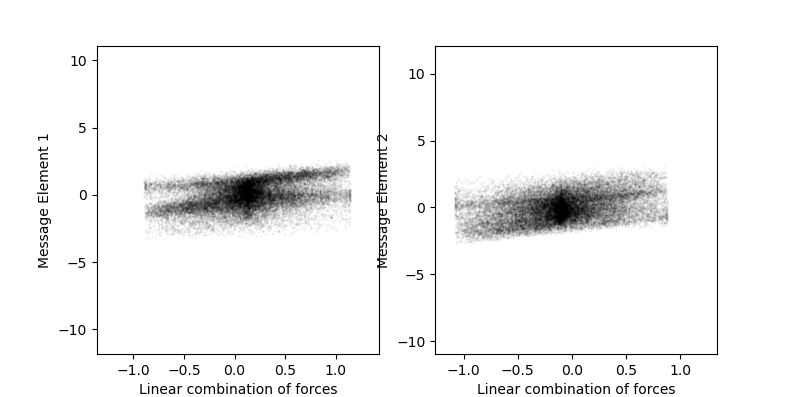
\includegraphics[width=\textwidth]{sp_res1.png}}\\
	\subfloat[][]{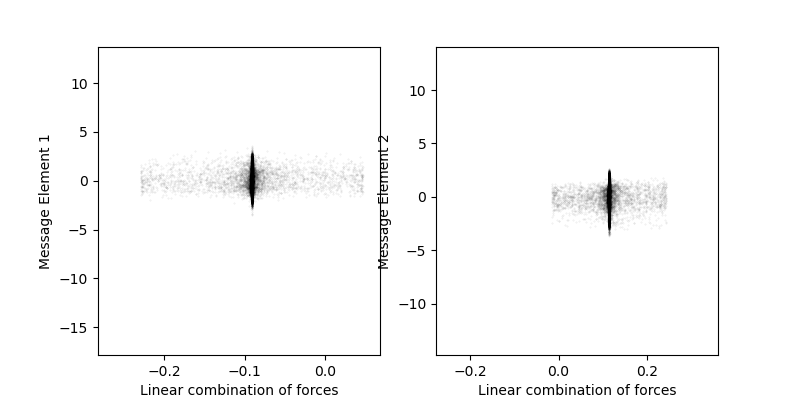
\includegraphics[width=\textwidth]{lj_res1.png}}
	\caption{\textbf{NOT DEFINITIVE IMAGES} Representative message-force plots of early epochs of training for spring potential (left) and Lennard Jones (right).}
	\label{fig:lincomb}
\end{figure}

As the animation in \cite{cranmer_discovering_2020} shows, as the network learns, the message-force graphs should show a better agreement between what is learned by the GNN and ground-truth.
In our case, as it is shown in fig \ref{fig:lincomb_last}, in the case of spring potential, the message-force plot has all the points on a vertical line, showing no correspondence between the learned results and ground-truth forces.
This could be caused by a tendency to overfit on the presented data, since loss is decreasing while test result are worse.

%\todo{sarebbe interessante vedere dei grafici della forza vs. distanza, ma visto che non riusciamo a mappare le componenti del messaggio alle forze, potremmo dare un'occhiata ai messaggi (norma?) vs. distanza}

Anyway, it is possible to notice a difference between the two potentials in Figure \ref{fig:lincomb}: in the case of Lennard Jones (Panel (b)), few points are outside the vertical line and they position in an horizontal cloud around it, while for the elastic potential (Panel (a)) most points are scattered around an horizontal cloud and a density increase can be observed in diagonal lines.

\begin{figure}[tp]
	\centering
	\subfloat[][]{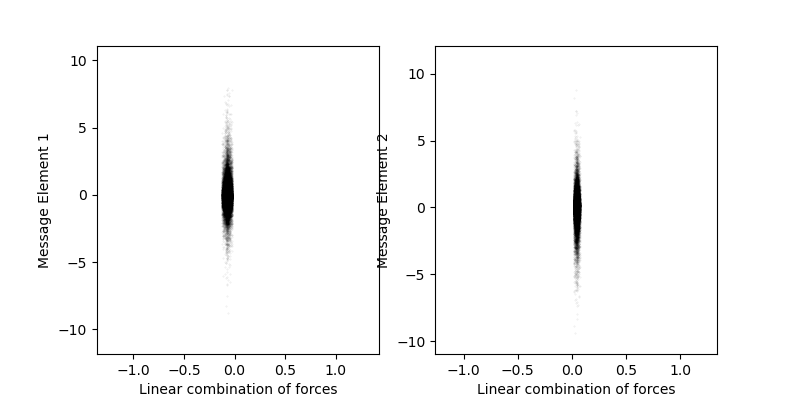
\includegraphics[width=\textwidth]{sp_reslast.png}}\\
	\subfloat[][]{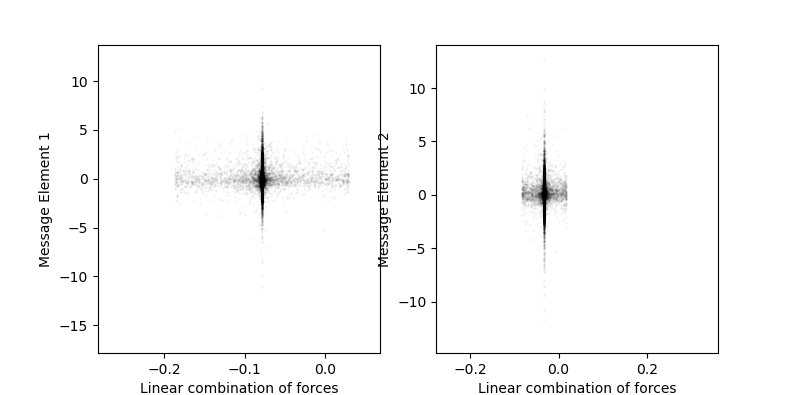
\includegraphics[width=\textwidth]{lj_reslast.png}}
	\caption{\textbf{NOT DEFINITIVE IMAGES} Representative message-force plots of last epoch of training for spring potential (left) and Lennard Jones (right).}
	\label{fig:lincomb_last}
\end{figure}


\section{Conclusions to Chapter 4}

Here we presented the preliminary version and results of a machine learning tool that predicts forces between interacting active particles, in the spirit of the ActiveNet system developed by \citeauthor{ruiz-garcia_discovering_2024}.

As shown in section \ref{4results}, more work is needed in order to make this tool work as expected.
In particular, training for longer with more simulation snapshots is certainly needed in order to get the right accuracy.
In reference paper, the problem of data amount is tackled comparing errors in cases with different simulation temperature.
It is clear how with higher temperature noise tends to increase and more data is needed in order to have accurate estimates of the self-propulsion and interaction forces.
In general, we can say that the amount of particles in our simulations (100) is pretty low if compared with what \citeauthor{ruiz-garcia_discovering_2024} have used (2500).
Knowing that the number of edges in an undirected graph is quadratic with the number of nodes, the number of total interactions to learn from is extremely low in our case if compared with the reference paper.

Retraining process with increasing threshold distance must be perfected, in order to get at the same level of the reference paper.
For all that was said in previous sections, it might be a good choice to start training with lower threshold distances, since \SI{20}{\um} already contains most of the significant interactions for the selected potentials. 

After making the training process work as desired, the next step is to retrain the network with snapshots taken from simulations with different potentials, in order to increase its generalization capability.

Moreover, testing with experimental data will need some more adjustments.
In an experimental setting, defects inherited from the fabrication process like stuck particles and particle clumps can make it harder for a machine learning tool to work properly.
In the case of experimental data collected in the Microscale Robotics Lab, it is hard to measure particles' orientation, since the two hemispheres of silica Janus particles are not clearly distinguishable, though a difference in color is noticeable.
Moreover, these particles are free to rotate in three dimensions and nothing prevents them from pointing one hemisphere to the microscope objective, not showing the separation line.
One workaround to this issue could be taking as particle's orientation the instantaneous angle that its trajectory forms, computing it between two consecutive instants.
This would be putting all the information about interactions inside self-propulsion, nonetheless if the two time scales are sufficiently different, one might be able to separate the two, leading to an accurate estimate of particles' orientation.
This approach needs some testing in simulations, when orientations are known, to understand its limitations and advantages.

We can state that these results, though certainly not satisfying, can be a starting point to further developments of this tool, getting it to work as expected in the case of active particles like those under investigation in the host laboratory.
With the potentials inferred from experiments, we would be able to model particles in a more accurate and complete way, to simulate them and use simulated data back in a simulation-driven inference fashion.
\end{document}